\documentclass[bahasa,10pt]{beamer}

\setlength{\parskip}{\smallskipamount}
\setlength{\parindent}{0pt}

\setbeamersize{text margin left=5pt, text margin right=5pt}

\usepackage{amsmath}
\usepackage{amssymb}
\usepackage{braket}

\usepackage{minted}
\newminted{python}{breaklines,fontsize=\footnotesize,texcomments=true}
\newminted{bash}{breaklines,fontsize=\footnotesize,texcomments=true}
\newminted{text}{breaklines,fontsize=\footnotesize,texcomments=true}

\definecolor{mintedbg}{rgb}{0.95,0.95,0.95}
\usepackage{mdframed}

%\BeforeBeginEnvironment{minted}{\begin{mdframed}[backgroundcolor=mintedbg]}
%\AfterEndEnvironment{minted}{\end{mdframed}}

\setcounter{secnumdepth}{3}
\setcounter{tocdepth}{3}

\makeatletter
%%%%%%%%%%%%%%%%%%%%%%%%%%%%%% Textclass specific LaTeX commands.
 % this default might be overridden by plain title style
 \newcommand\makebeamertitle{\frame{\maketitle}}%
 % (ERT) argument for the TOC
 \AtBeginDocument{%
   \let\origtableofcontents=\tableofcontents
   \def\tableofcontents{\@ifnextchar[{\origtableofcontents}{\gobbletableofcontents}}
   \def\gobbletableofcontents#1{\origtableofcontents}
 }

\makeatother

\usepackage{babel}

\begin{document}


\title{Pengenalan ASE (Atomic Simulation Environment)}
\author{Fadjar Fathurrahman}
\institute{
Program Studi Teknik Fisika \\
Divisi Komputasi Pusat Penelitian Nanosains dan Nanoteknologi \\
Institut Teknologi Bandung
}
\date{23 April 2018}

\frame{\titlepage}

\begin{frame}
\frametitle{Atomic Simulation Environment}

Merupakan pustaka Python untuk melakukan mempermudah \textit{workflow}
dalam teknik simulasi berbasis atom seperti DFT dan MD.

Mempermudah \textit{scripting}

\end{frame}



\begin{frame}[fragile]
\frametitle{Membuat struktur atomik}

\begin{pythoncode}
from ase import Atoms
atoms = Atoms("Ni4", [(0, 0, 0), (2.0, 0, 0), (0.0, 2.0, 0), (2.0, 2.0, 0)],
               cell=[5, 5, 5])
atoms.set_pbc([True,True,True])  # anggap sebagai struktur periodik
\end{pythoncode}

Simpan struktur atom dalam beberapa format:
\begin{pythoncode}
atoms.write("Ni4.xyz")  # extended XYZ format
atoms.write("Ni4.xsf")  # Xcrysden format
\end{pythoncode}

\end{frame}



\begin{frame}[fragile]
\frametitle{Visualisasi sederhana}

Visualisasi dengan \texttt{ase-gui}:
\begin{pythoncode}
import ase.visualize
ase.visualize(atoms)
\end{pythoncode}

Simpan hasil visualisasi dalam format EPS (\textit{encapsulated postscript})
\begin{pythoncode}
ase.visualize.write("Ni4.eps", atoms, format="eps")
# ase.io.write (dengan signature fungsi yang sama) juga dapat digunakan
\end{pythoncode}

{\centering
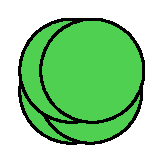
\includegraphics[scale=0.4]{Ni4.eps}
\par}

\end{frame}


\begin{frame}[fragile]
\frametitle{Contoh}

\begin{pythoncode}
from ase import Atoms, Atom
from ase.io import write
b = 7.1
atoms = Atoms([Atom("C", [0., 0., 0.]),
               Atom("O", [1.1, 0., 0.])],
               cell=[[b, b, 0.],
                     [b, 0., b],
                     [0., b, b]])
print("Volume = {0:1.0f} Ang^3".format(atoms.get_volume()))
atoms.center()        # translasi atoms ke tengah sel
write("CO-in-fcc.eps", atoms, show_unit_cell=2)
\end{pythoncode}

{\centering
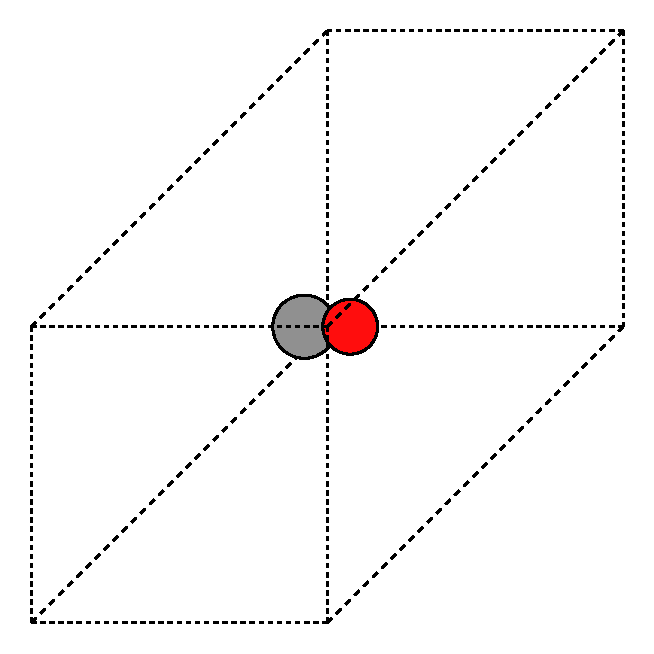
\includegraphics[scale=0.4]{CO-in-fcc.eps}
\par}

\end{frame}


\begin{frame}
\frametitle{ASE calculator}

Dapat menggunakan program eksternal:

\end{frame}



\begin{frame}
\frametitle{NEB}


\end{frame}



\end{document}

